% ----------------------------------------------------------
\chapter{Paleta de cores da UnB}\label{anx:coresunb}
% ----------------------------------------------------------

A paleta de cores da UnB, disponível na \cpageref{marcaunb.1} a seguir, foi extraída do \emph{manual de identidade visual}\footnote{Disponível em \url{http://marca.unb.br}} da Universidade.

Note que, de acordo com a ABNT, a principal diferença entre anexo e apêndice é que os apêndices são textos criados pelo próprio autor para complementar sua argumentação, enquanto os anexos são documentos criados por terceiros, e usados pelo autor.

\cleardoublepage

\newcounter{includepdfpage} % para referenciar no texto páginas pdf incluídas

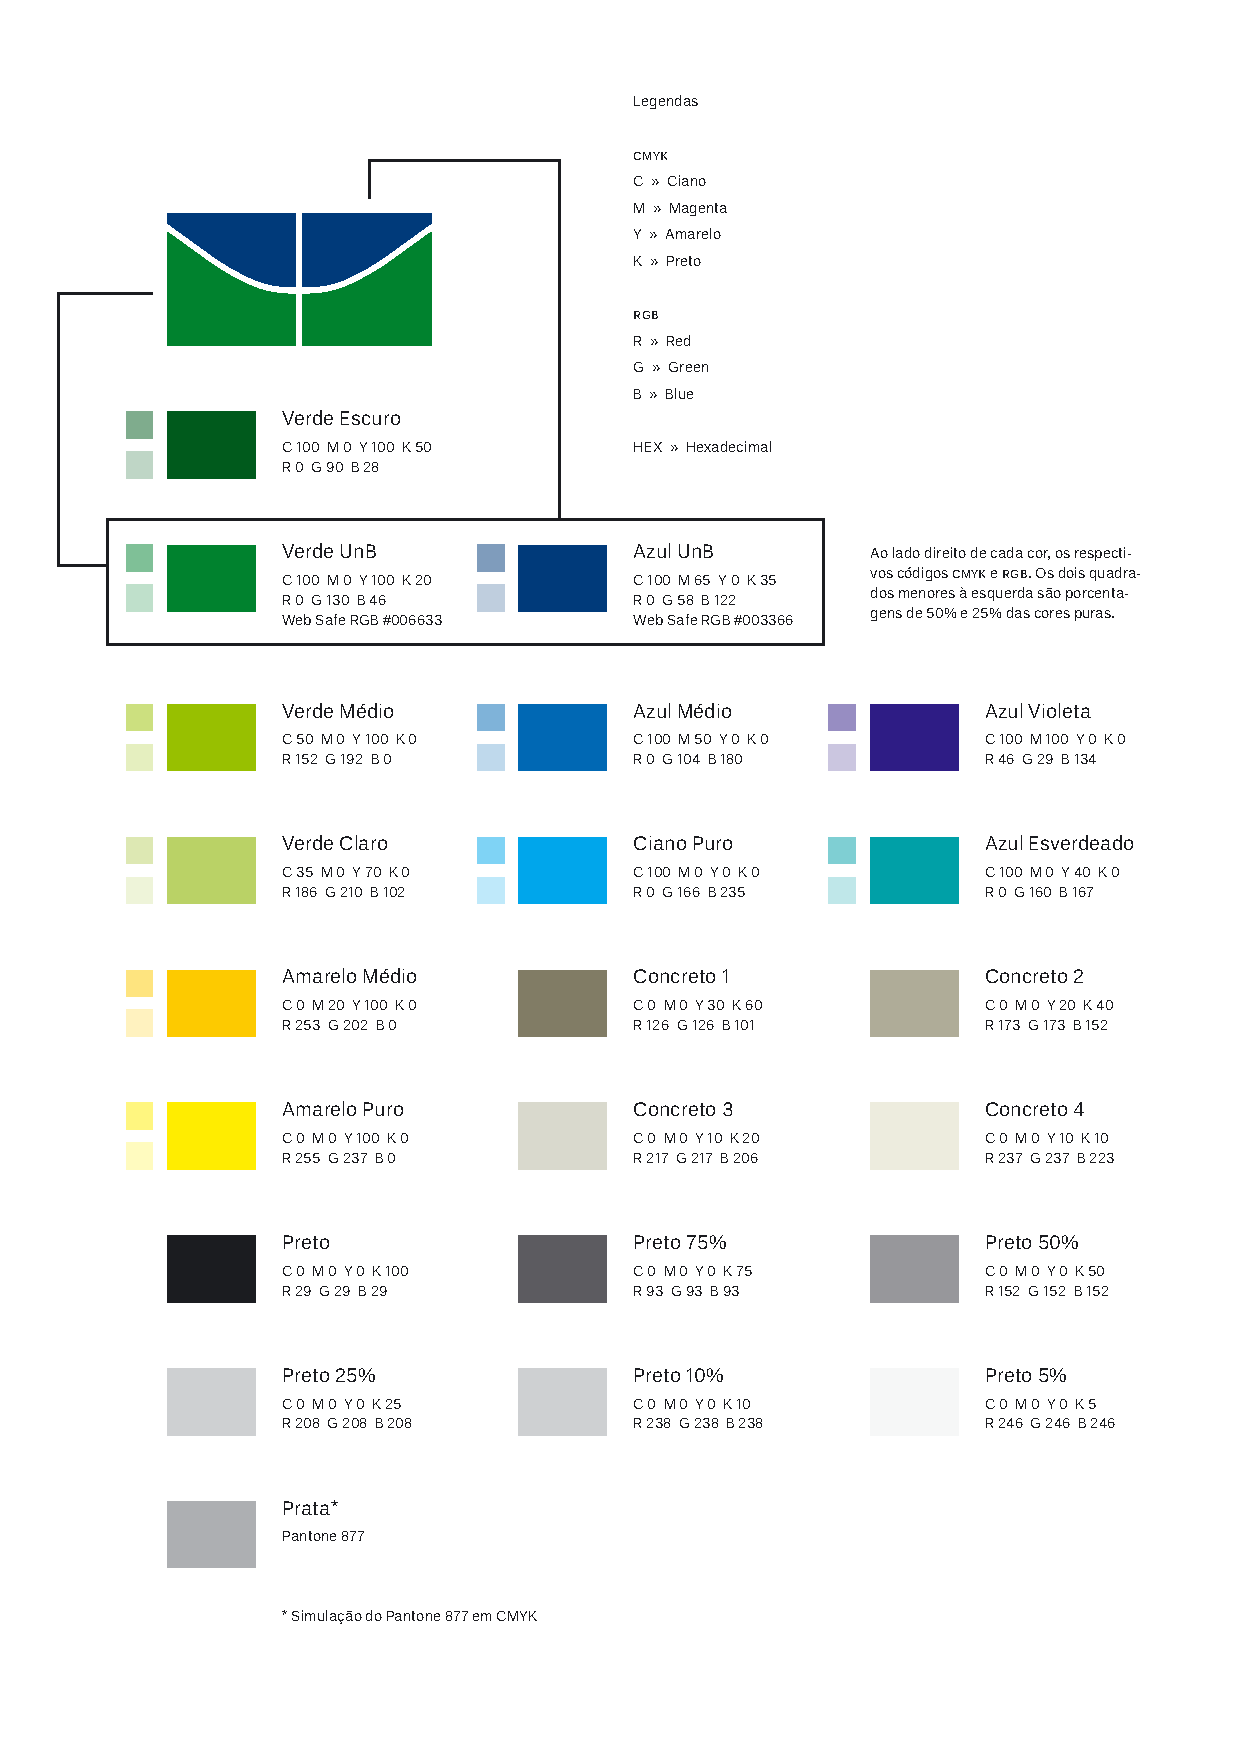
\includepdf[
    pages=-, % intervalo das páginas do arquivo pdf que serão incluídas
    scale=1, % controla o tamanho da página inserida
    pagecommand={\thispagestyle{plain} % imprime o número da página
    \refstepcounter{includepdfpage} % conta a página incluída
    \label{marcaunb.\theincludepdfpage} % marcaunb.n, n número da página
    },
    ]{unbtex-example/figuras/coresunb}

\cleardoublepage